\documentclass[conference]{IEEEtran}
\IEEEoverridecommandlockouts
% The preceding line is only needed to identify funding in the first footnote. If that is unneeded, please comment it out.
\usepackage{cite}
\usepackage{amsmath,amssymb,amsfonts}
\usepackage{algorithmic}
\usepackage{graphicx}
\usepackage{graphics}
\usepackage{textcomp}
\usepackage{xcolor}
\usepackage{tikz}
\usepackage[english]{cleveref}

\usetikzlibrary{shapes,arrows}

\usepackage{pgfplots}
%\usepackage[top=30pt,bottom=40pt,left=46pt,right=48pt]{geometry}
\def\BibTeX{{\rm B\kern-.05em{\sc i\kern-.025em b}\kern-.08em
    T\kern-.1667em\lower.7ex\hbox{E}\kern-.125emX}}

\begin{document}
\begin{titlepage}
	\title{Report: Image Processing and Computer Vision 2018}
  	\author{\IEEEauthorblockN{Florian Bauer}
			\IEEEauthorblockA{\textit{School of Computer Science} \\
			\textit{University of Bristol}\\
					Bristol, UK\\
					ya18048@bristol.ac.uk}
			\and
			\IEEEauthorblockN{Ruben Powar}
			\IEEEauthorblockA{\textit{School of Computer Science} \\
			\textit{University of Bristol}\\
			Bristol, UK\\
			wz18202@bristol.ac.uk}
			}
			\maketitle
\end{titlepage}
\newpage

\section{Subtask 1}

\subsection{Result Images}


\begin{figure}[ht!]
\centering
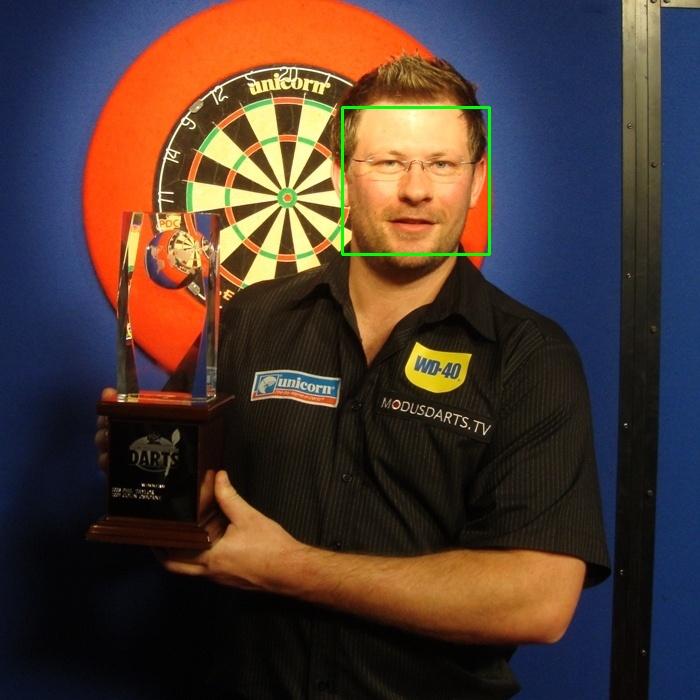
\includegraphics[width=60mm]{img/Viola_Jones_Faces/face_detection4.jpg}
\caption{Image face4.jpg | $F1 = 100\%$ \label{img_face_4}}
\end{figure}

\begin{figure}[ht!]
\centering
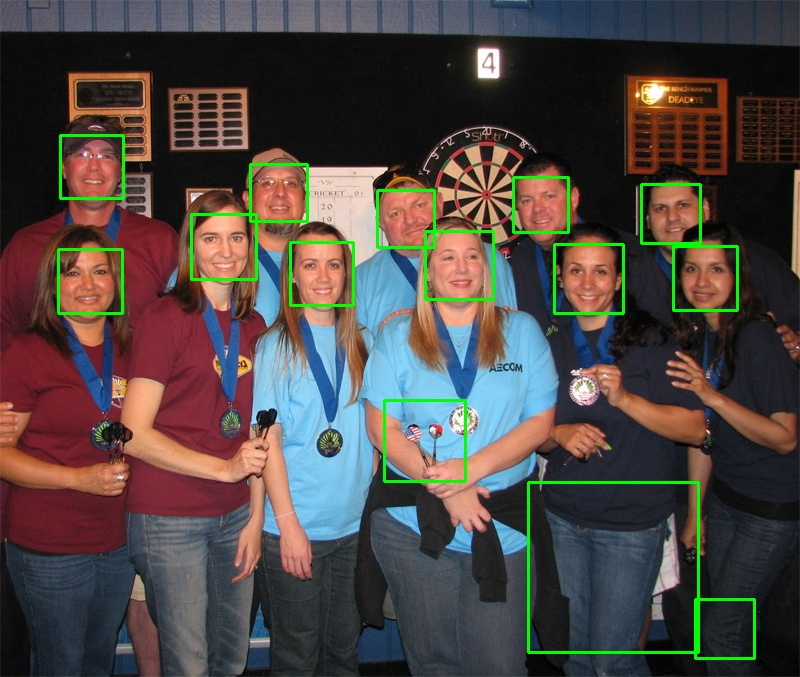
\includegraphics[width=60mm]{img/Viola_Jones_Faces/face_detection5.jpg}
\caption{Image face5.jpg | $F1 = 88\%$ \label{img_face_5}}
\end{figure}

\begin{figure}[ht!]
\centering
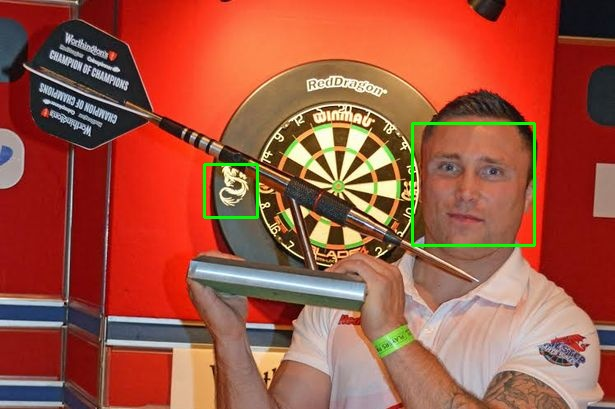
\includegraphics[width=60mm]{img/Viola_Jones_Faces/face_detection13.jpg}
\caption{Image face13.jpg | $F1 = 66.67\%$ \label{img_face_13}}
\end{figure}

\begin{figure}[ht!]
\centering
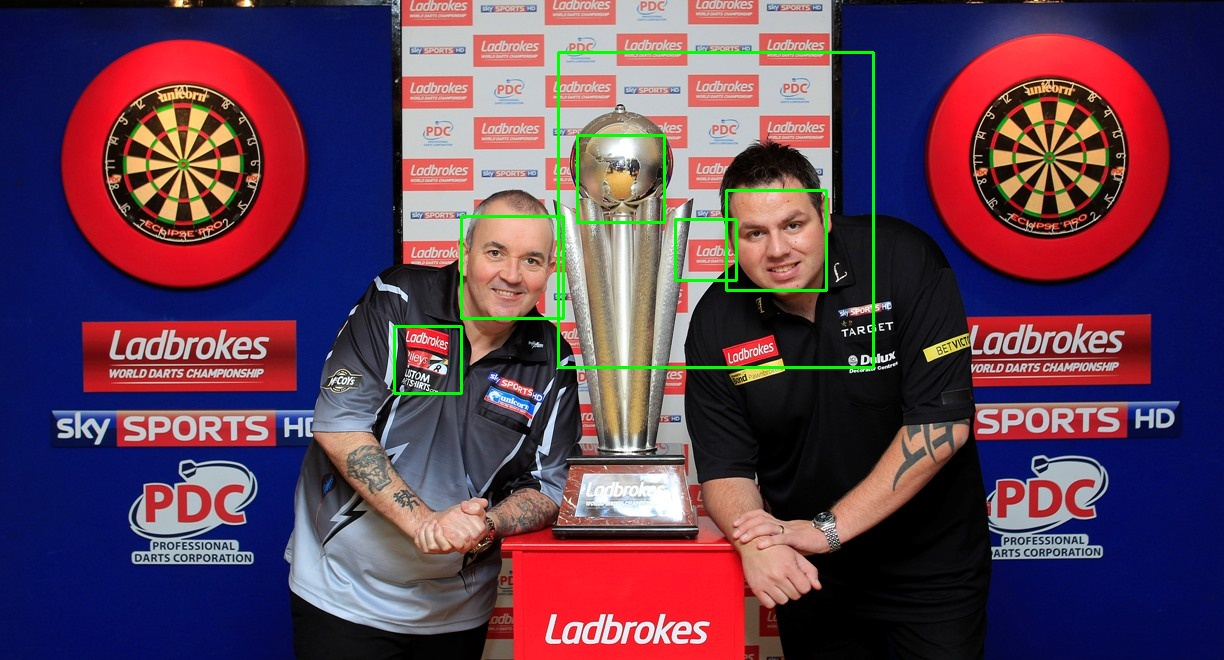
\includegraphics[width=60mm]{img/Viola_Jones_Faces/face_detection14.jpg}
\caption{Image face14.jpg | $F1 = 50\%$ \label{img_face_14}}
\end{figure}

\begin{figure}[ht!]
\centering
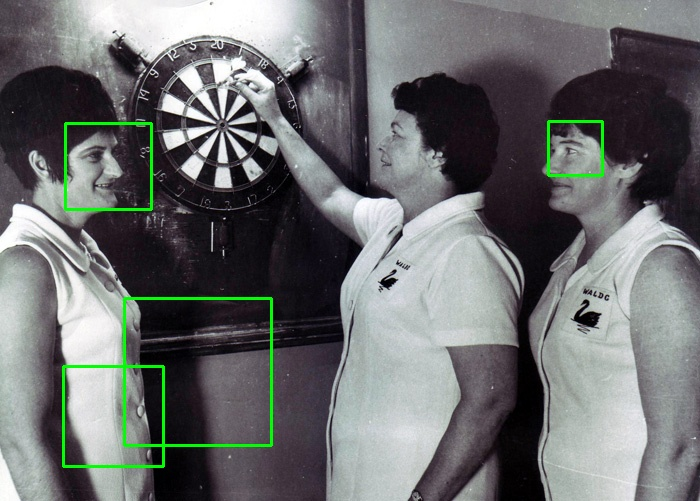
\includegraphics[width=60mm]{img/Viola_Jones_Faces/face_detection15.jpg}
\caption{Image face15.jpg | $F1 = 57.14\%$ \label{img_face_15}}
\end{figure}

\subsection{TPR and F1-score calculation}

Calculating the true positive rate:
\[TPR = \frac{TP}{P} = \frac{TP}{TP+FN}\]
where :\\
$TPR$ = True positive rate \\
$TP$ = The number of cases correctly recognised \\
$P$ = The number of actual positive cases in the data\\
$FN$ = The number of false negatives, or the number of actual true cases not recognised\\

dart5.jpg TPR = 
\[\frac{11}{11+0} = 1 \therefore 100\%\]

dart15.jpg TPR = 
\[\frac{2}{2+1} = 0.\dot{6} \therefore 66.\dot{6}\%\]


The TPR is independent of the false positive rate. Consider a face detection task where we have $x$ faces to detect $(A = \{face_{1} \ldots face_{x}\}$ and a hypothetical model that produces a set of detected faces $B$ comprised of all $y$ possible contiguous combinations of pixel areas. $A \subset B$, however it also contains $y-x$ false positive detections. In this case the model has a TPR of 100\%, however a potentially much lower precision. This hypothetical model is always possible, regardless of input, therefore a TPR of 100\% is always possible.



$$F_{1} = \left(\frac{TPR{-1} \cdot PRECISION^{-1}}{2} \right) ^{-1}$$
$$= 2 \cdot \frac{PRECISION \cdot TPR}{PRECISION + TPR}$$
$$ PRECISION = \frac{TP}{TP + FP}$$
where :
$FP$ = False positive rate

\newpage

\section{Subtask 2}

\subsection{TPR vs FPR Scatter Plot}

\begin{center}
	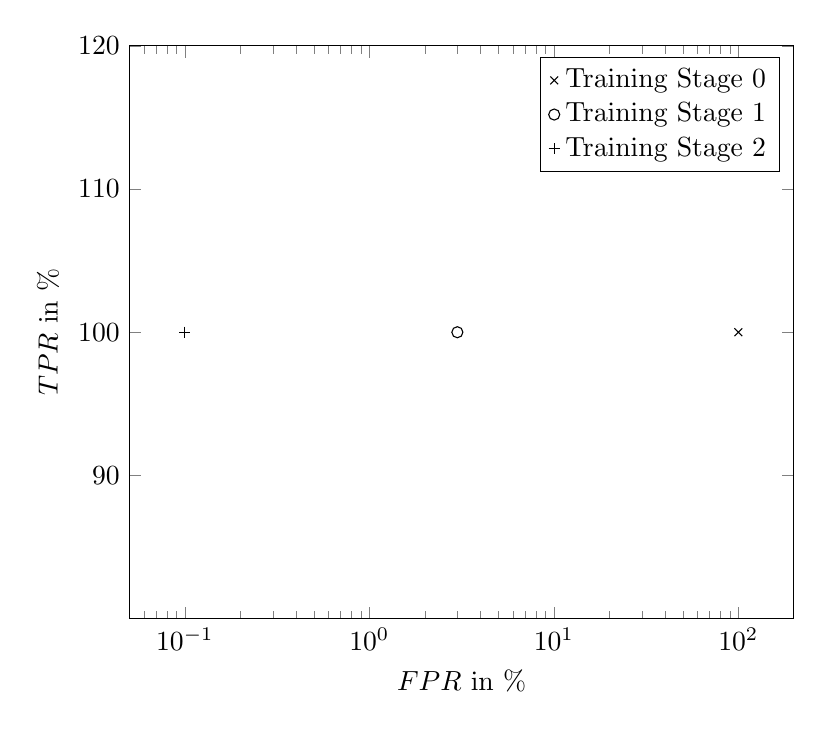
\begin{tikzpicture}
		\pgfplotsset{
			scale only axis,
		}

		\begin{axis}[
			xmode=log,
		xlabel=$FPR$ in \%,
		ylabel=$TPR$ in \%,
		]
		\addplot[only marks, mark=x]
		coordinates{ % plot 1 data set
			(100,100)
		}; \label{training stage 0}
		\addplot[only marks, mark=o]
		coordinates{ % plot 1 data set
			(3,100)
		}; \label{training stage 1}
		\addplot[only marks, mark=+]
		coordinates{ % plot 1 data set
			(0.1,100)
		}; \label{training stage 2}

		% plot 1 legend entry
		\addlegendimage{/pgfplots/refstyle=plot_one}
		\addlegendentry{Training Stage 0}
		\addlegendentry{Training Stage 1}
		\addlegendentry{Training Stage 2}
		\end{axis}

	\end{tikzpicture}
\end{center}

As training progresses from stage 0 to 2 we see that the \textit{true positive rate} (TPR) appears to remain constant. This is due to being parametrised with a minimum hit rate of 0.999, essentially ensuring that all dartboards are detected while the algorithm attempts to reduce the number of false positives. We can see that \textit{false positive rate} decreases at an exponential rate between each of the training stages.

\subsection{F1-Scores for Dartboards}

\begin{figure}[ht!]
	\centering
	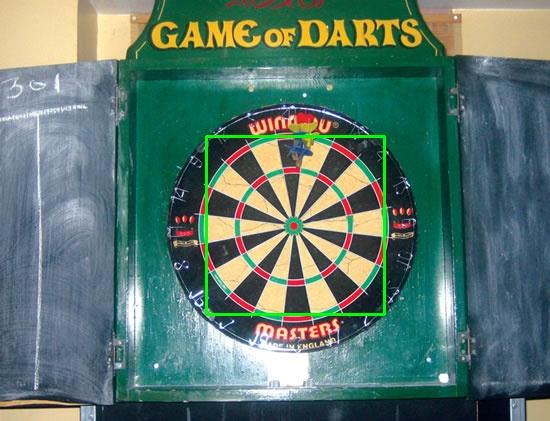
\includegraphics[width=50mm]{img/Viola_Jones_Darts/detected_dart1.jpg}
	\caption{Image dart1.jpg \label{img_dart_1}}
\end{figure}

\begin{figure}[ht!]
	\centering
	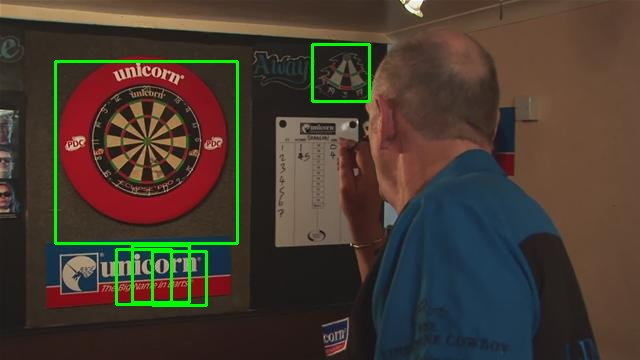
\includegraphics[width=50mm]{img/Viola_Jones_Darts/detected_dart2.jpg}
	\caption{Image dart2.jpg \label{img_dart_2}}
\end{figure}

\begin{figure}[ht!]
	\centering
	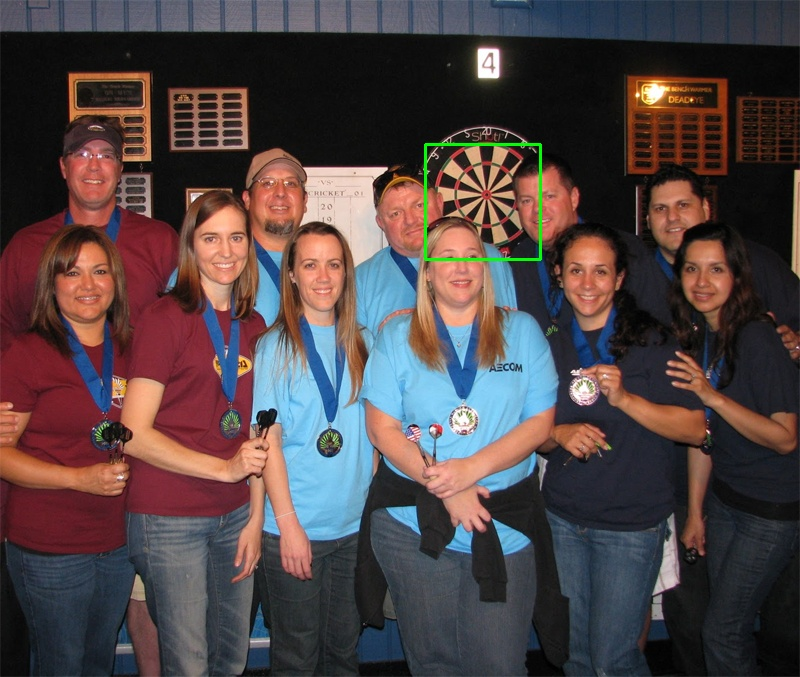
\includegraphics[width=50mm]{img/Viola_Jones_Darts/detected_dart5.jpg}
	\caption{Image dart5.jpg \label{img_dart_5}}
\end{figure}

\begin{figure}[ht!]
	\centering
	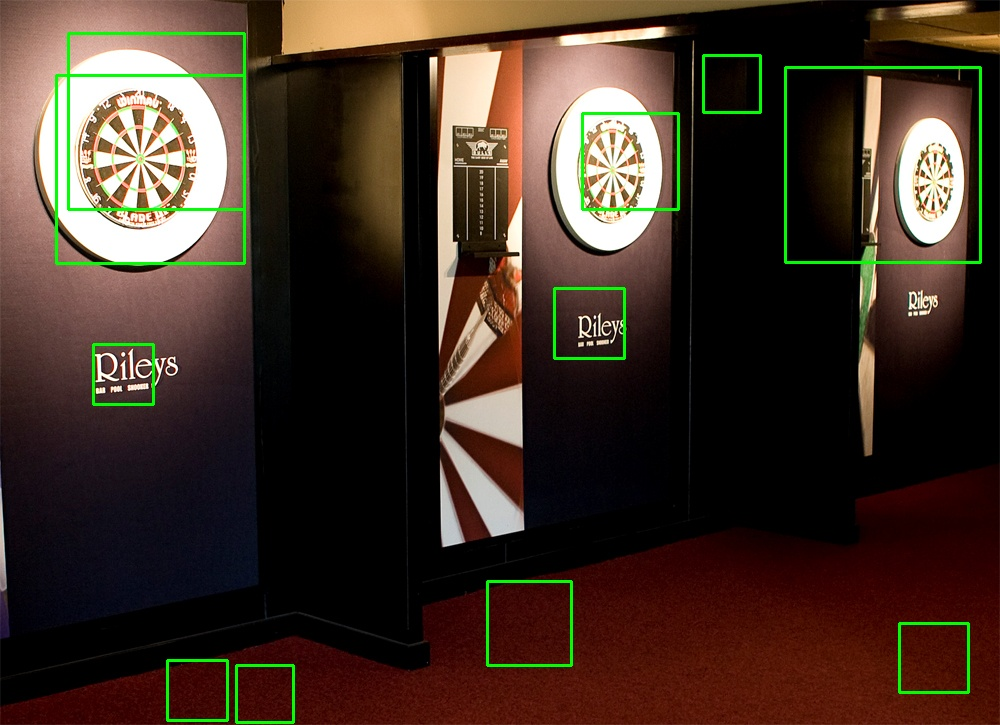
\includegraphics[width=50mm]{img/Viola_Jones_Darts/detected_dart10.jpg}
	\caption{Image dart10.jpg \label{img_dart_10}}
\end{figure}

\begin{center}
	\begin{tabular}{| l | l | l | l |}
		\hline
		Image & F1-Score \\ \hline
	    0 & 100\% \\ \hline
		1 & 100\% \\ \hline
		2 & 33.33\% \\ \hline
		3 &  50\%\\ \hline
		4 & 50\% \\ \hline
		5 & 100\% \\ \hline
		6 & 66.67\% \\ \hline
		7 & 28.57\% \\ \hline
		8 & 66.67\% \\ \hline
		9 & 66.67\% \\ \hline
		10 & 42.86\% \\ \hline
		11 & 0\% \\ \hline
		12 & 66.67\% \\ \hline
		13 & 66.67\% \\ \hline
		14 & 44.44\% \\ \hline
		15 & 100\% \\ \hline
		average & 61.32\% \\ \hline
	\end{tabular}
\end{center}

In the table above the F1-Scores for Viola-Jones model trained on dartboards have been calculated. This model produces a reasonable true positive rate, managing to detect dartboards in the majority of test images. The model however also has a tendency to produce many false positives resulting in a decrease in F1-Scores for certain test cases. The model struggles with some partly obscured dartboards as well as identifying a single dartboard multiple times.


\newpage

\section{Subtask 3}

\subsection{Images for Hough Space, Gradient Magnitude, and Final Result}

\begin{figure}[ht!]
	\centering
	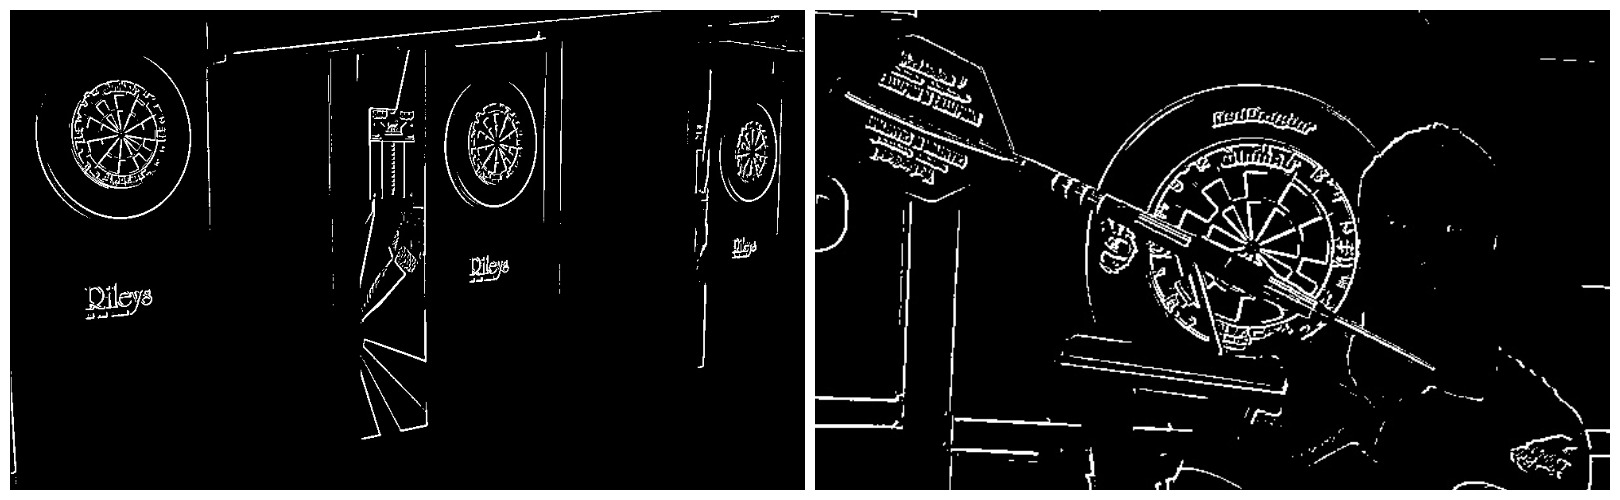
\includegraphics[width=90mm]{img/Task3_Images/threshold_dart.jpg}
	\caption{Thresholded Gradient Magnitude for images dart10.jpg and dart13.jpg}
	\label{ThresholdGM}
\end{figure}


\begin{figure}[ht!]
	\centering
	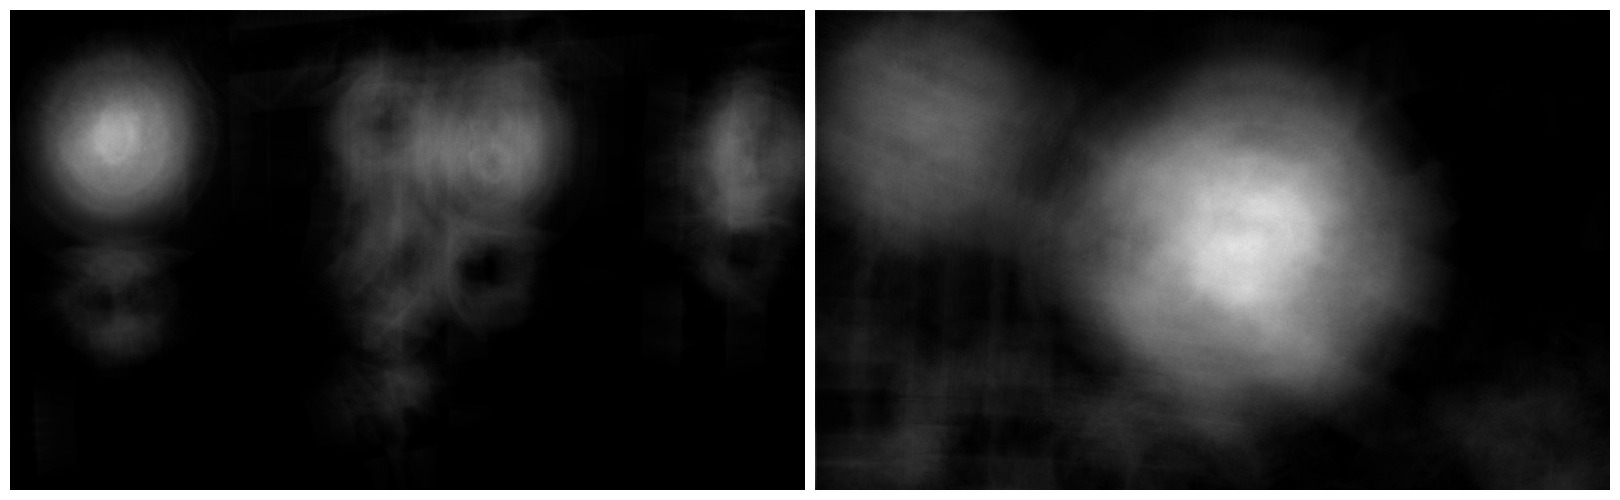
\includegraphics[width=90mm]{img/Task3_Images/houghspace_dart.jpg}
	\caption{Hough Space for images dart10.jpg and dart13.jpg}
\end{figure}

\begin{figure}[ht!]
	\centering
	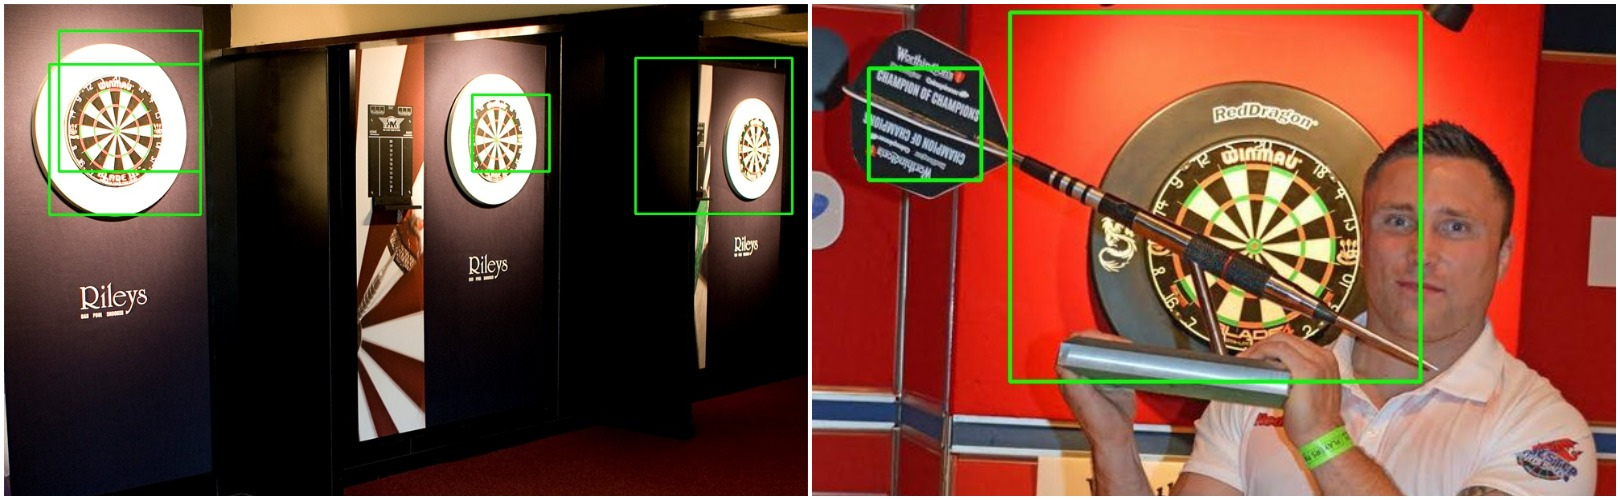
\includegraphics[width=90mm]{img/Task3_Images/detected_dart.jpg}
	\caption{Final Detections for images dart10.jpg and dart13.jpg}
\end{figure}

\subsection{Evaluation of Detector}

\begin{center}
	\begin{tabular}{| l | l | l | l |}
		\hline
		Image & F1-Score & Precision & Recall \\ \hline
		0 & 100\% & 100\% & 100\% \\ \hline
		1 & 100\% & 100\% & 100\% \\ \hline
		2 & 100\% & 100\% & 100\% \\ \hline
		3 &  0\% & 0\% & 0\% \\ \hline
		4 & 66.67\% & 50\% & 100\% \\ \hline
		5 & 100\% & 100\% & 100\% \\ \hline
		6 & 100\%  & 100\% & 100\% \\ \hline
		7 & 50\% & 33.33\% & 100\%\\ \hline
		8 & 100\% & 100\% & 100\% \\ \hline
		9 & 100\% & 100\% & 100\% \\ \hline
		10 & 85.71\% & 75\% & 100\% \\ \hline
		11 & 0\% & 0\% & 0\% \\ \hline
		12 & 100\% & 100\% & 100\% \\ \hline
		13 & 66.67\% & 50\% & 100\% \\ \hline
		14 & 57.14\% & 40\% & 100\% \\ \hline
		15 & 100\% & 100\% & 100\%\\ \hline
		average & 76.60\% & 71.77\% & 87.5\% \\ \hline
	\end{tabular}
\end{center}

\begin{itemize}
	\item[+] False positive rate strongly decreases due to a requirement of a positive from both \textbf{Viola-Jones}, and \textbf{Hough Circle Detection}
	\item[+] There is an improvement of 16 percentage points over regular Viola-Jones (A \texttildelow 25\% improvement).
	\item[-] A small number of false negatives was introduced (Viola-Jones produced close to no false negatives, dependent on the trained model)
	\item[-] Like Viola-Jones, overlapping detection rectangles result in an increase in the false positive rate.
\end{itemize}

\subsection{Evidence of Combined Hough Transform and Viola-Jones}

\tikzstyle{block} = [rectangle, draw, fill=blue!20, text width=5em, text centered, rounded corners, minimum height=4em]
\tikzstyle{line} = [draw, -latex']
\tikzstyle{cloud} = [draw, ellipse,fill=red!20, node distance=3cm,
minimum height=2em]

\begin{tikzpicture}[node distance = 2cm, auto]
	    \node [block] (ViolaJones) {ViolaJones};
	    \node [cloud, left of=ViolaJones] (Train) {Training Data};
	    \node [cloud, right of=ViolaJones] (Input) {Input Image};
	    \node [block, below of=ViolaJones] (Model) {Combined Model};
        \node [block, below of=Input] (Hough) {Hough Circle Detector};
        \node [cloud, below of=Model] (Output) {Detected Dart Boards};
        \path [line] (ViolaJones) -- (Model);
        \path [line] (Hough) -- (Model);
        \path [line,dashed] (Model) -- (Output);
        \path [line,dashed] (Train) -- (ViolaJones);
        \path [line,dashed] (Input) -- (ViolaJones);
        \path [line,dashed] (Input) -- (Hough);
	    
\end{tikzpicture}

\begin{itemize}
	\item Viola-Jones is first trained using the training data as input.
	\item Viola-Jones receives an test image as input and returns detected dart boards.
	\item The Hough Circle Detector receives the same input image after pre-processing.
	\item This pre-processing produces a gradient magnitude image which is then thresholded to generate a black and white image on which the Hough space is calculated.
	\item In order to reduce memory usage rather than using a three dimensional Hough space, for each radius size a Hough space is calculated, circles are detected, and the resulting Hough space is added to a two dimensional accumulated Hough space. 
	\item All detected dart boards are cross referenced against the Hough detector's circles.
	\item If a Viola-Jones detected board contains no circle it is disregarded as a false positive.
	\item Conversely, if the board contains one or more circles the Viola-Jones prediction is considered to have been confirmed.
	\item The decision to confirm Viola-Jones using detected Hough circles and not vice versa is due to the following: 
	\begin{itemize}
		\item Viola-Jones has a comparatively lower false positive rate.
		\item Viola-Jones has a near 100\% true positive rate
	\end{itemize}
\end{itemize}

\newpage
\section{Subtask 4}

\subsection{Rationale}
\begin{itemize}
	\item In order to avoid false positives produced by dartboards being detected multiple times with Viola-Jones overlapping boards have been consolidated into one.
	\item This works because of the assumption that boards would not be expected to overlap or lie within the edge of another in reality due to their positioning: being mounted typically on solid walls, and being of fixed size.
\end{itemize}

\textbf{Future Improvements}
The following improvements have been partially implemented and included in the submitted code, however are not in use for the final model.
\begin{itemize}
	\item Add an implementation of a Hough lines detector detecting line intersections. 
	\item Any point at or near which multiple lines intersect is potentially the centre of a dart board.
	\item The efficacy of this method is largely independent of the angle at which the dartboard is viewed.
	\item Adding this detection of potential dartboard centres to the combined model can be done in a similar way to the addition of the circle detector, due to how the combined model is constructed.
\end{itemize}

In our given implementation of the Hough circles algorithm we are using as input a thresholded gradient magnitude image--an example of which can be seen in \cref{ThresholdGM}. This has allowed for a model that runs in a reasonable time-frame for each given image (a matter of seconds). However, in the case that the input images are much larger in size this method may become infeasible. An optimisation that has the potential to greatly reduce runtime while still producing sufficiently accurate output is to include gradient direction in the Hough Transform.

\subsection{Images showing aspects of the final technique}

\begin{figure}[ht!]
	\centering
	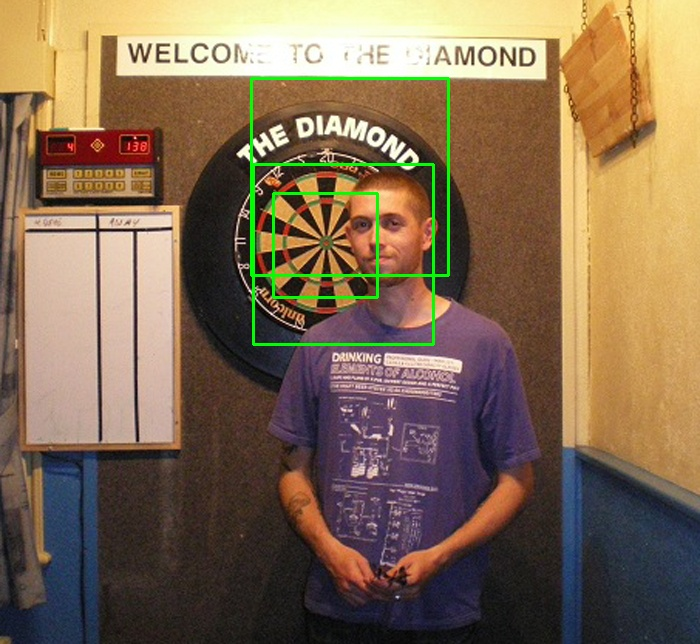
\includegraphics[width=45mm]{img/Task4_Images/detected_dart7_unmerged.jpg}
	\caption{The detected dartboards for image dart7.jpg without merging of overlapping dartboards.}
	\label{Unmerged VJ-Hough}
\end{figure}

\begin{figure}[ht!]
	\centering
	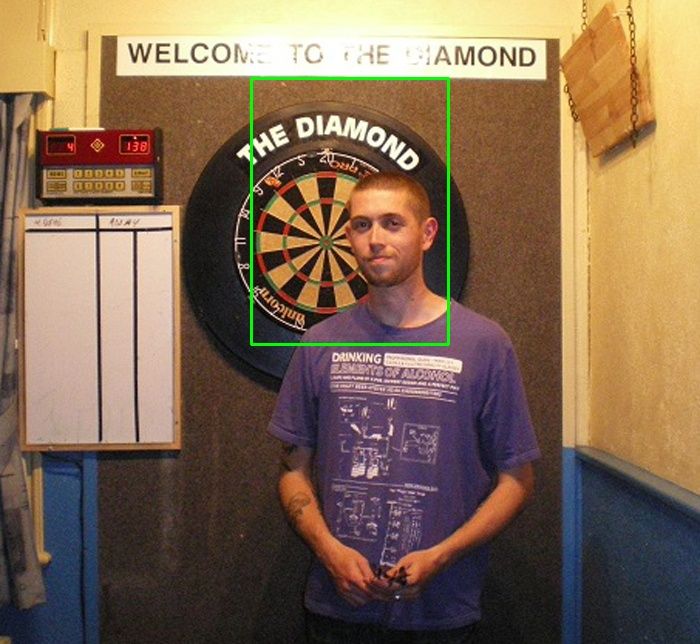
\includegraphics[width=45mm]{img/Task4_Images/detected_dart7_merged.jpg}
	\caption{The detected dartboards for image dart7.jpg with merging of overlapping dartboards.}
	\label{Merged VJ-Hough}
\end{figure}

As we can see in \cref{Unmerged VJ-Hough}, our unoptimised model, there are three bounding rectangles representing recognised dart boards. This model shows zero false negatives, however 2/3 of the recognitions are superfluous. By combining these overlapping boxes, assuming that in reality overlapping boxes represent multiple instances of the same dart board predicted we can refine the model to produce only one bounding box as shown in \cref{Merged VJ-Hough}, thus improving the output of the model.


\subsection{Final F1-Scores}
\begin{center}
	\begin{tabular}{| l | l | l | l |}
		\hline
		Image & F1-Score & Precision & Recall \\ \hline
		0 & 100\% & 100\% & 100\% \\ \hline
		1 & 100\% & 100\% & 100\% \\ \hline
		2 & 100\% & 100\% & 100\% \\ \hline
		3 &  0\% & 0\% & 0\% \\ \hline
		4 & 100\% & 100\% & 100\% \\ \hline
		5 & 100\% & 100\% & 100\% \\ \hline
		6 & 100\%  & 100\% & 100\% \\ \hline
		7 & 100\% & 100\% & 100\%\\ \hline
		8 & 100\% & 100\% & 100\% \\ \hline
		9 & 66.67\% & 50\% & 100\% \\ \hline
		10 & 100\% & 100\% & 100\% \\ \hline
		11 & 0\% & 0\% & 0\% \\ \hline
		12 & 100\% & 100\% & 100\% \\ \hline
		13 & 100\% & 100\% & 100\% \\ \hline
		14 & 66.67\% & 50\% & 100\% \\ \hline
		15 & 100\% & 100\% & 100\%\\ \hline
		average & 83.33\% & 81.25\% & 87.5\% \\ \hline
	\end{tabular}
\end{center}

\subsection{Final Comments}
\begin{itemize}
	\item Our final model overall shows better performance than any of the previous models. 
	
	\item When compared to the naive combination model of Viola-Jones and Hough circles we have achieved an identical Recall, but a significantly higher F1-Score and Precision.
	
	\item This by extension means that it outperforms both Viola-Jones, and Hough circles independently. 
	
	\item It should be noted that the efficacy of the model can vary due to the robustness of the trained Viola-Jones model.
	
	\item Because of this there tends to be some trade-off between correctly detecting difficult boards(i.e. where the image shows a large amount of noise, or where the board is partly obscured) and producing false positives. Some examples of this are boards three and eleven which in the model we evaluated were entirely undetected.
	
\end{itemize}

Our final implementation was able to achieve 100\% F1-Score, Recall, and Precision on twelve out of the sixteen test images, representing a considerably accurate trained model.

\end{document}